\PassOptionsToPackage{unicode=true}{hyperref} % options for packages loaded elsewhere
\PassOptionsToPackage{hyphens}{url}
%
\documentclass[]{article}
\usepackage{lmodern}
\usepackage{amssymb,amsmath}
\usepackage{ifxetex,ifluatex}
\usepackage{fixltx2e} % provides \textsubscript
\ifnum 0\ifxetex 1\fi\ifluatex 1\fi=0 % if pdftex
  \usepackage[T1]{fontenc}
  \usepackage[utf8]{inputenc}
  \usepackage{textcomp} % provides euro and other symbols
\else % if luatex or xelatex
  \usepackage{unicode-math}
  \defaultfontfeatures{Ligatures=TeX,Scale=MatchLowercase}
\fi
% use upquote if available, for straight quotes in verbatim environments
\IfFileExists{upquote.sty}{\usepackage{upquote}}{}
% use microtype if available
\IfFileExists{microtype.sty}{%
\usepackage[]{microtype}
\UseMicrotypeSet[protrusion]{basicmath} % disable protrusion for tt fonts
}{}
\IfFileExists{parskip.sty}{%
\usepackage{parskip}
}{% else
\setlength{\parindent}{0pt}
\setlength{\parskip}{6pt plus 2pt minus 1pt}
}
\usepackage{hyperref}
\hypersetup{
            pdftitle={Project1},
            pdfauthor={Kathleen Strybos},
            pdfborder={0 0 0},
            breaklinks=true}
\urlstyle{same}  % don't use monospace font for urls
\usepackage[margin=1in]{geometry}
\usepackage{color}
\usepackage{fancyvrb}
\newcommand{\VerbBar}{|}
\newcommand{\VERB}{\Verb[commandchars=\\\{\}]}
\DefineVerbatimEnvironment{Highlighting}{Verbatim}{commandchars=\\\{\}}
% Add ',fontsize=\small' for more characters per line
\usepackage{framed}
\definecolor{shadecolor}{RGB}{248,248,248}
\newenvironment{Shaded}{\begin{snugshade}}{\end{snugshade}}
\newcommand{\AlertTok}[1]{\textcolor[rgb]{0.94,0.16,0.16}{#1}}
\newcommand{\AnnotationTok}[1]{\textcolor[rgb]{0.56,0.35,0.01}{\textbf{\textit{#1}}}}
\newcommand{\AttributeTok}[1]{\textcolor[rgb]{0.77,0.63,0.00}{#1}}
\newcommand{\BaseNTok}[1]{\textcolor[rgb]{0.00,0.00,0.81}{#1}}
\newcommand{\BuiltInTok}[1]{#1}
\newcommand{\CharTok}[1]{\textcolor[rgb]{0.31,0.60,0.02}{#1}}
\newcommand{\CommentTok}[1]{\textcolor[rgb]{0.56,0.35,0.01}{\textit{#1}}}
\newcommand{\CommentVarTok}[1]{\textcolor[rgb]{0.56,0.35,0.01}{\textbf{\textit{#1}}}}
\newcommand{\ConstantTok}[1]{\textcolor[rgb]{0.00,0.00,0.00}{#1}}
\newcommand{\ControlFlowTok}[1]{\textcolor[rgb]{0.13,0.29,0.53}{\textbf{#1}}}
\newcommand{\DataTypeTok}[1]{\textcolor[rgb]{0.13,0.29,0.53}{#1}}
\newcommand{\DecValTok}[1]{\textcolor[rgb]{0.00,0.00,0.81}{#1}}
\newcommand{\DocumentationTok}[1]{\textcolor[rgb]{0.56,0.35,0.01}{\textbf{\textit{#1}}}}
\newcommand{\ErrorTok}[1]{\textcolor[rgb]{0.64,0.00,0.00}{\textbf{#1}}}
\newcommand{\ExtensionTok}[1]{#1}
\newcommand{\FloatTok}[1]{\textcolor[rgb]{0.00,0.00,0.81}{#1}}
\newcommand{\FunctionTok}[1]{\textcolor[rgb]{0.00,0.00,0.00}{#1}}
\newcommand{\ImportTok}[1]{#1}
\newcommand{\InformationTok}[1]{\textcolor[rgb]{0.56,0.35,0.01}{\textbf{\textit{#1}}}}
\newcommand{\KeywordTok}[1]{\textcolor[rgb]{0.13,0.29,0.53}{\textbf{#1}}}
\newcommand{\NormalTok}[1]{#1}
\newcommand{\OperatorTok}[1]{\textcolor[rgb]{0.81,0.36,0.00}{\textbf{#1}}}
\newcommand{\OtherTok}[1]{\textcolor[rgb]{0.56,0.35,0.01}{#1}}
\newcommand{\PreprocessorTok}[1]{\textcolor[rgb]{0.56,0.35,0.01}{\textit{#1}}}
\newcommand{\RegionMarkerTok}[1]{#1}
\newcommand{\SpecialCharTok}[1]{\textcolor[rgb]{0.00,0.00,0.00}{#1}}
\newcommand{\SpecialStringTok}[1]{\textcolor[rgb]{0.31,0.60,0.02}{#1}}
\newcommand{\StringTok}[1]{\textcolor[rgb]{0.31,0.60,0.02}{#1}}
\newcommand{\VariableTok}[1]{\textcolor[rgb]{0.00,0.00,0.00}{#1}}
\newcommand{\VerbatimStringTok}[1]{\textcolor[rgb]{0.31,0.60,0.02}{#1}}
\newcommand{\WarningTok}[1]{\textcolor[rgb]{0.56,0.35,0.01}{\textbf{\textit{#1}}}}
\usepackage{graphicx,grffile}
\makeatletter
\def\maxwidth{\ifdim\Gin@nat@width>\linewidth\linewidth\else\Gin@nat@width\fi}
\def\maxheight{\ifdim\Gin@nat@height>\textheight\textheight\else\Gin@nat@height\fi}
\makeatother
% Scale images if necessary, so that they will not overflow the page
% margins by default, and it is still possible to overwrite the defaults
% using explicit options in \includegraphics[width, height, ...]{}
\setkeys{Gin}{width=\maxwidth,height=\maxheight,keepaspectratio}
\setlength{\emergencystretch}{3em}  % prevent overfull lines
\providecommand{\tightlist}{%
  \setlength{\itemsep}{0pt}\setlength{\parskip}{0pt}}
\setcounter{secnumdepth}{0}
% Redefines (sub)paragraphs to behave more like sections
\ifx\paragraph\undefined\else
\let\oldparagraph\paragraph
\renewcommand{\paragraph}[1]{\oldparagraph{#1}\mbox{}}
\fi
\ifx\subparagraph\undefined\else
\let\oldsubparagraph\subparagraph
\renewcommand{\subparagraph}[1]{\oldsubparagraph{#1}\mbox{}}
\fi

% set default figure placement to htbp
\makeatletter
\def\fps@figure{htbp}
\makeatother


\title{Project1}
\author{Kathleen Strybos}
\date{2/28/2020}

\begin{document}
\maketitle

\hypertarget{project-1-exploratory-data-analysis-food-insecurity-and-demographics-in-texas-counties}{%
\subsection{Project 1 Exploratory Data Analysis: Food Insecurity and
Demographics in Texas
Counties}\label{project-1-exploratory-data-analysis-food-insecurity-and-demographics-in-texas-counties}}

\#Introduction \emph{The two datasets that were chosen for this project
center around health across counties in Texas. The ``health'' dataset
contains 15 different variables for different health measures across
counties in Texas. These variables include the names of Texas counties,
average life expectancy, the rate at which members of the population are
in frequent mental distress, the rate of diabetes prevalence, rates of
both food insecurity across the county and the rate of limited food
access in the counties, rates of the amount of uninsured adults and
children, average household incomes across three races: white, black and
hispanic, free/reduced lunch rates among school-aged children,
urbanization status indicators of whether the counties are rural or
urban, and the border status of the counties, which indicates whether or
not they are on the border. This data was acquired at the County Health
Rankings and Roadmaps website funded by the Robert Wood Johnson
Foundation Program.}

\emph{The other dataset, called ``mapmeal'' was acquired through Feeding
America. This dataset contains 4 variables, including county names in
Texas, the food insecurity rate across the entire county's population,
child food insecurity rate more specifically, and the average cost per
meal in a county. These two datasets are interesting to me because I am
going into the field of healthcare. I hope to become a pediatrician, so
data centered around children's health, family dynamics and
accessibility to resources is a point of interest for me, as it pertains
to my future career. I expect to see that there is an association
between child food insecurity rate and the percentage of children in a
county on free and reduced lunch. The underlying variable within this
situation likely has to do with household income as well. Many of the
variables in these datasets pertain to socioeconomic status within the
counties, and I expect to see associations that are typical for certain
socioeconomic statuses.}

\begin{Shaded}
\begin{Highlighting}[]
\KeywordTok{library}\NormalTok{(tidyverse)}
\NormalTok{health=}\StringTok{ }\KeywordTok{read.csv}\NormalTok{(}\StringTok{"health.csv"}\NormalTok{)}
\NormalTok{mapmeal=}\StringTok{ }\KeywordTok{read.csv}\NormalTok{(}\StringTok{"mapmeal.csv"}\NormalTok{)}
\KeywordTok{glimpse}\NormalTok{(health)}
\end{Highlighting}
\end{Shaded}

\begin{verbatim}
## Observations: 254
## Variables: 15
## $ County                     <fct> Anderson, Andrews, Angelina, Aransas, Ar...
## $ lifeexpectancy             <dbl> 73.8, 76.8, 76.3, 76.9, 77.0, 72.4, 78.3...
## $ frequentmentaldistressrate <int> 11, 10, 13, 12, 10, 10, 11, 11, 13, 11, ...
## $ diabeticrate               <int> 11, 9, 14, 14, 11, 11, 12, 10, 10, 11, 1...
## $ foodinsecurerate           <int> 19, 9, 20, 16, 15, 14, 9, 16, 10, 15, 13...
## $ limitedaccessfoodrate      <int> 15, 12, 11, 20, 5, 20, 8, 3, 4, 13, 11, ...
## $ uninsuredadultrate         <int> 21, 22, 24, 24, 20, 17, 23, 22, 34, 20, ...
## $ uninsuredchildrenrate      <int> 11, 12, 10, 13, 13, 12, 9, 11, 13, 13, 1...
## $ Household.Income           <int> 42412, 63451, 45318, 46970, 58311, 55337...
## $ householdiincome_black     <int> 24427, 38359, 28509, NA, NA, NA, 72827, ...
## $ householdincome_hispanic   <int> 37635, 66319, 41673, 43302, 34375, 15025...
## $ householdincome_white      <int> 48013, 73648, 51631, 45496, 65504, 64737...
## $ free_reduced_lunch_percent <int> 61, 42, 66, 56, 32, 51, 63, 54, 81, 54, ...
## $ urbanization               <fct> Rural, Rural, Rural, Urban, Urban, Urban...
## $ border_status              <fct> Non-Border, Non-Border, Non-Border, Non-...
\end{verbatim}

\begin{Shaded}
\begin{Highlighting}[]
\KeywordTok{glimpse}\NormalTok{(mapmeal)}
\end{Highlighting}
\end{Shaded}

\begin{verbatim}
## Observations: 254
## Variables: 4
## $ county                  <fct> Anderson, Andrews, Angelina, Aransas, Arche...
## $ foodinsecurityrate      <dbl> 0.182, 0.084, 0.189, 0.165, 0.140, 0.131, 0...
## $ childfoodinsecurityrate <dbl> 0.234, 0.184, 0.253, 0.263, 0.201, 0.203, 0...
## $ costpermeal             <dbl> 2.75, 2.94, 2.94, 2.95, 2.83, 3.06, 2.78, 3...
\end{verbatim}

\hypertarget{tidying-rearranging-widelong}{%
\subsection{Tidying: Rearranging
Wide/Long}\label{tidying-rearranging-widelong}}

\begin{Shaded}
\begin{Highlighting}[]
\CommentTok{#Untidying "health" data#}
\NormalTok{health1 <-health }\OperatorTok\StringTok{ }\KeywordTok{pivot_longer}\NormalTok{(}\KeywordTok{c}\NormalTok{(}\StringTok{"uninsuredadultrate"}\NormalTok{, }\StringTok{"uninsuredchildrenrate"}\NormalTok{), }
\DataTypeTok{names_to =} \StringTok{"uninsured"}\NormalTok{, }\DataTypeTok{values_to =} \StringTok{"percentage uninsured"}\NormalTok{) }\OperatorTok\StringTok{ }\KeywordTok{glimpse}\NormalTok{()}
\end{Highlighting}
\end{Shaded}

\begin{verbatim}
## Observations: 508
## Variables: 15
## $ County                     <fct> Anderson, Anderson, Andrews, Andrews, An...
## $ lifeexpectancy             <dbl> 73.8, 73.8, 76.8, 76.8, 76.3, 76.3, 76.9...
## $ frequentmentaldistressrate <int> 11, 11, 10, 10, 13, 13, 12, 12, 10, 10, ...
## $ diabeticrate               <int> 11, 11, 9, 9, 14, 14, 14, 14, 11, 11, 11...
## $ foodinsecurerate           <int> 19, 19, 9, 9, 20, 20, 16, 16, 15, 15, 14...
## $ limitedaccessfoodrate      <int> 15, 15, 12, 12, 11, 11, 20, 20, 5, 5, 20...
## $ Household.Income           <int> 42412, 42412, 63451, 63451, 45318, 45318...
## $ householdiincome_black     <int> 24427, 24427, 38359, 38359, 28509, 28509...
## $ householdincome_hispanic   <int> 37635, 37635, 66319, 66319, 41673, 41673...
## $ householdincome_white      <int> 48013, 48013, 73648, 73648, 51631, 51631...
## $ free_reduced_lunch_percent <int> 61, 61, 42, 42, 66, 66, 56, 56, 32, 32, ...
## $ urbanization               <fct> Rural, Rural, Rural, Rural, Rural, Rural...
## $ border_status              <fct> Non-Border, Non-Border, Non-Border, Non-...
## $ uninsured                  <chr> "uninsuredadultrate", "uninsuredchildren...
## $ `percentage uninsured`     <int> 21, 11, 22, 12, 24, 10, 24, 13, 20, 13, ...
\end{verbatim}

\begin{Shaded}
\begin{Highlighting}[]
\CommentTok{#Tidying "health" data#}
\NormalTok{health1 }\OperatorTok\StringTok{ }\KeywordTok{spread}\NormalTok{(}\DataTypeTok{key=}\StringTok{"uninsured"}\NormalTok{, }\DataTypeTok{value=} \StringTok{"percentage uninsured"}\NormalTok{)}
\end{Highlighting}
\end{Shaded}

\begin{verbatim}
## # A tibble: 254 x 15
##    County lifeexpectancy frequentmentald~ diabeticrate foodinsecurerate
##    <fct>           <dbl>            <int>        <int>            <int>
##  1 Ander~           73.8               11           11               19
##  2 Andre~           76.8               10            9                9
##  3 Angel~           76.3               13           14               20
##  4 Arans~           76.9               12           14               16
##  5 Archer           77                 10           11               15
##  6 Armst~           72.4               10           11               14
##  7 Atasc~           78.3               11           12                9
##  8 Austin           79.1               11           10               16
##  9 Bailey           78.4               13           10               10
## 10 Bande~           80.3               11           11               15
## # ... with 244 more rows, and 10 more variables: limitedaccessfoodrate <int>,
## #   Household.Income <int>, householdiincome_black <int>,
## #   householdincome_hispanic <int>, householdincome_white <int>,
## #   free_reduced_lunch_percent <int>, urbanization <fct>, border_status <fct>,
## #   uninsuredadultrate <int>, uninsuredchildrenrate <int>
\end{verbatim}

\begin{Shaded}
\begin{Highlighting}[]
\CommentTok{#Untidying "mapmeal" data#}
\NormalTok{mapmeal1<-}\StringTok{ }\NormalTok{mapmeal }\OperatorTok\StringTok{ }\KeywordTok{pivot_longer}\NormalTok{(}\KeywordTok{c}\NormalTok{(}\StringTok{"foodinsecurityrate"}\NormalTok{, }\StringTok{"childfoodinsecurityrate"}\NormalTok{), }
\DataTypeTok{names_to=} \StringTok{"food insecurity"}\NormalTok{, }
\DataTypeTok{values_to=} \StringTok{"percentage food insecure"}\NormalTok{) }\OperatorTok\StringTok{ }\KeywordTok{glimpse}\NormalTok{()}
\end{Highlighting}
\end{Shaded}

\begin{verbatim}
## Observations: 508
## Variables: 4
## $ county                     <fct> Anderson, Anderson, Andrews, Andrews, An...
## $ costpermeal                <dbl> 2.75, 2.75, 2.94, 2.94, 2.94, 2.94, 2.95...
## $ `food insecurity`          <chr> "foodinsecurityrate", "childfoodinsecuri...
## $ `percentage food insecure` <dbl> 0.182, 0.234, 0.084, 0.184, 0.189, 0.253...
\end{verbatim}

\begin{Shaded}
\begin{Highlighting}[]
\CommentTok{#Tidying "health" data#}
\NormalTok{mapmeal1 }\OperatorTok\StringTok{ }\KeywordTok{spread}\NormalTok{(}\DataTypeTok{key=}\StringTok{"food insecurity"}\NormalTok{, }\DataTypeTok{value=} \StringTok{"percentage food insecure"}\NormalTok{)}
\end{Highlighting}
\end{Shaded}

\begin{verbatim}
## # A tibble: 254 x 4
##    county    costpermeal childfoodinsecurityrate foodinsecurityrate
##    <fct>           <dbl>                   <dbl>              <dbl>
##  1 Anderson         2.75                   0.234              0.182
##  2 Andrews          2.94                   0.184              0.084
##  3 Angelina         2.94                   0.253              0.189
##  4 Aransas          2.95                   0.263              0.165
##  5 Archer           2.83                   0.201              0.14 
##  6 Armstrong        3.06                   0.203              0.131
##  7 Atascosa         2.78                   0.212              0.088
##  8 Austin           3.12                   0.228              0.147
##  9 Bailey           2.98                   0.243              0.112
## 10 Bandera          3.4                    0.255              0.145
## # ... with 244 more rows
\end{verbatim}

\emph{For the tidying/untidying portion of this project, I decided to
untidy the columns in the ``health'' dataset concerned with the rate of
the adult population that is uninsured and the rate of the child
population that is uninsured. I created a new dataset called ``health1''
to house these modifications. I used pivot\_longer() to accomplish the
untidying since my ``health'' data was already tidy. With this result, I
could see both the adult and child uninsurance rates in one column for a
particular county. For the ``mapmeal'' dataset, I decided to untidy the
columns for child food insecurity rate and overall food insecurity rate
using the pivot\_longer() function, since my data was already tidy. I
created a new dataset called ``mapmeal1'' to house these modifications.
With this result, I could see both the overall population's and
children's food insecurity rates for a particular county.}

\emph{To re-tidy my datasets, I used the spread() function. For the
``health1'' dataset, I filled in ``uninsured'' and ``percentage
uninsured'' for key and value, respectively to re-tidy my data. For the
``mapmeal1'' I filled in ``food insecurity'' and ``percentage food
insecure'' for key and value, respectively. This allowed me to re-tidy
my data.}

\#Joining/Merging

\begin{Shaded}
\begin{Highlighting}[]
\NormalTok{joindata <-health }\OperatorTok\StringTok{ }\KeywordTok{full_join}\NormalTok{(mapmeal, }\DataTypeTok{by=}\KeywordTok{c}\NormalTok{(}\StringTok{"County"}\NormalTok{=}\StringTok{ "county"}\NormalTok{))}
\NormalTok{joindata }\OperatorTok\StringTok{ }\KeywordTok{glimpse}\NormalTok{()}
\end{Highlighting}
\end{Shaded}

\begin{verbatim}
## Observations: 254
## Variables: 18
## $ County                     <fct> Anderson, Andrews, Angelina, Aransas, Ar...
## $ lifeexpectancy             <dbl> 73.8, 76.8, 76.3, 76.9, 77.0, 72.4, 78.3...
## $ frequentmentaldistressrate <int> 11, 10, 13, 12, 10, 10, 11, 11, 13, 11, ...
## $ diabeticrate               <int> 11, 9, 14, 14, 11, 11, 12, 10, 10, 11, 1...
## $ foodinsecurerate           <int> 19, 9, 20, 16, 15, 14, 9, 16, 10, 15, 13...
## $ limitedaccessfoodrate      <int> 15, 12, 11, 20, 5, 20, 8, 3, 4, 13, 11, ...
## $ uninsuredadultrate         <int> 21, 22, 24, 24, 20, 17, 23, 22, 34, 20, ...
## $ uninsuredchildrenrate      <int> 11, 12, 10, 13, 13, 12, 9, 11, 13, 13, 1...
## $ Household.Income           <int> 42412, 63451, 45318, 46970, 58311, 55337...
## $ householdiincome_black     <int> 24427, 38359, 28509, NA, NA, NA, 72827, ...
## $ householdincome_hispanic   <int> 37635, 66319, 41673, 43302, 34375, 15025...
## $ householdincome_white      <int> 48013, 73648, 51631, 45496, 65504, 64737...
## $ free_reduced_lunch_percent <int> 61, 42, 66, 56, 32, 51, 63, 54, 81, 54, ...
## $ urbanization               <fct> Rural, Rural, Rural, Urban, Urban, Urban...
## $ border_status              <fct> Non-Border, Non-Border, Non-Border, Non-...
## $ foodinsecurityrate         <dbl> 0.182, 0.084, 0.189, 0.165, 0.140, 0.131...
## $ childfoodinsecurityrate    <dbl> 0.234, 0.184, 0.253, 0.263, 0.201, 0.203...
## $ costpermeal                <dbl> 2.75, 2.94, 2.94, 2.95, 2.83, 3.06, 2.78...
\end{verbatim}

\emph{I chose to join my ``health'' and ``mapmeal'' datasets using a
full join. By using a full join, I was able to keep all of my
observations. Even though there are NAs where there are no observations,
this was not due to the joining process. Because both datasets were
joined on the basis of Texas counties, all of the data alligned really
well, hence the reason a full join was the appropriate choice. The only
NAs that are present in my data were there when I retrieved the data.
The NA observations are not there because there was never any
information retrieved for a particular variable in a given column. There
were not any cases dropped. I know this because there were 254 rows in
the ``health'' dataset, and there are 254 rows in the ``joindata.'' This
means that there were not any cases dropped.}

\#Wrangling

\begin{Shaded}
\begin{Highlighting}[]
\CommentTok{#Using Core dplyr Functions}
\NormalTok{smalljoindata<-joindata }\OperatorTok\StringTok{ }\KeywordTok{mutate}\NormalTok{(}\DataTypeTok{foodcost_peryear=}\NormalTok{ (costpermeal}\OperatorTok{*}\DecValTok{3}\OperatorTok{*}\DecValTok{365}\NormalTok{)) }\OperatorTok
\KeywordTok{filter}\NormalTok{(lifeexpectancy }\OperatorTok{>}\DecValTok{80}\NormalTok{) }\OperatorTok\StringTok{ }
\KeywordTok{select}\NormalTok{(County,lifeexpectancy, uninsuredadultrate,}
\NormalTok{foodcost_peryear, Household.Income,}
\NormalTok{border_status, urbanization, diabeticrate) }\OperatorTok\StringTok{ }
\KeywordTok{arrange}\NormalTok{(lifeexpectancy) }\OperatorTok\StringTok{ }\KeywordTok{group_by}\NormalTok{(border_status)}
\NormalTok{joindata }\OperatorTok\StringTok{ }\KeywordTok{summarize_all}\NormalTok{(}\ControlFlowTok{function}\NormalTok{(x)}\KeywordTok{sum}\NormalTok{(}\KeywordTok{is.na}\NormalTok{(x)))}
\end{Highlighting}
\end{Shaded}

\begin{verbatim}
##   County lifeexpectancy frequentmentaldistressrate diabeticrate
## 1      0             17                          0            0
##   foodinsecurerate limitedaccessfoodrate uninsuredadultrate
## 1                0                     1                  0
##   uninsuredchildrenrate Household.Income householdiincome_black
## 1                     0                0                     96
##   householdincome_hispanic householdincome_white free_reduced_lunch_percent
## 1                       11                    11                          1
##   urbanization border_status foodinsecurityrate childfoodinsecurityrate
## 1            0             0                  0                       0
##   costpermeal
## 1           0
\end{verbatim}

\begin{Shaded}
\begin{Highlighting}[]
\CommentTok{#Creating Summary Statistics}
\NormalTok{smalljoindata }\OperatorTok\StringTok{ }\KeywordTok{summarize}\NormalTok{(}\DataTypeTok{mean_lifeexpectancy=}
\KeywordTok{mean}\NormalTok{(lifeexpectancy, }\DataTypeTok{na.rm =}\NormalTok{ T), }
\DataTypeTok{sd_foodcost_year=}\KeywordTok{sd}\NormalTok{(foodcost_peryear, }\DataTypeTok{na.rm =}\NormalTok{ T), }
\DataTypeTok{IQR_householdincome=}\KeywordTok{IQR}\NormalTok{(Household.Income,}
\DataTypeTok{na.rm =}\NormalTok{ T), }\DataTypeTok{number_counties=}\KeywordTok{n_distinct}\NormalTok{(County),}
\DataTypeTok{min_householdincome=}\KeywordTok{min}\NormalTok{(Household.Income), }
\DataTypeTok{cor_foodcost_diabetes=}\KeywordTok{cor}\NormalTok{(foodcost_peryear,}
\NormalTok{diabeticrate), }
\DataTypeTok{median_uninsuredadultrate=}\KeywordTok{median}\NormalTok{(uninsuredadultrate))}
\end{Highlighting}
\end{Shaded}

\begin{verbatim}
## # A tibble: 2 x 8
##   border_status mean_lifeexpect~ sd_foodcost_year IQR_householdin~
##   <fct>                    <dbl>            <dbl>            <dbl>
## 1 Border                    83.6             364.            5292.
## 2 Non-Border                81.2             159.           30948.
## # ... with 4 more variables: number_counties <int>, min_householdincome <int>,
## #   cor_foodcost_diabetes <dbl>, median_uninsuredadultrate <dbl>
\end{verbatim}

\begin{Shaded}
\begin{Highlighting}[]
\NormalTok{smalljoindata }\OperatorTok\StringTok{ }
\KeywordTok{group_by}\NormalTok{(urbanization, border_status) }\OperatorTok
\KeywordTok{summarize}\NormalTok{(}\KeywordTok{max}\NormalTok{(lifeexpectancy))}
\end{Highlighting}
\end{Shaded}

\begin{verbatim}
## # A tibble: 4 x 3
## # Groups:   urbanization [2]
##   urbanization border_status `max(lifeexpectancy)`
##   <fct>        <fct>                         <dbl>
## 1 Rural        Border                         90.6
## 2 Rural        Non-Border                     81.6
## 3 Urban        Border                         86.4
## 4 Urban        Non-Border                     83
\end{verbatim}

\begin{Shaded}
\begin{Highlighting}[]
\NormalTok{smalljoindata }\OperatorTok\StringTok{ }\KeywordTok{group_by}\NormalTok{(urbanization) }\OperatorTok
\KeywordTok{summarize}\NormalTok{(}\KeywordTok{n_distinct}\NormalTok{(County))}
\end{Highlighting}
\end{Shaded}

\begin{verbatim}
## # A tibble: 2 x 2
##   urbanization `n_distinct(County)`
##   <fct>                       <int>
## 1 Rural                          12
## 2 Urban                          16
\end{verbatim}

\begin{Shaded}
\begin{Highlighting}[]
\NormalTok{smalljoindata }\OperatorTok\StringTok{ }\KeywordTok{group_by}\NormalTok{(urbanization,}
\NormalTok{border_status) }\OperatorTok
\KeywordTok{summarize}\NormalTok{(}\KeywordTok{median}\NormalTok{(diabeticrate))}
\end{Highlighting}
\end{Shaded}

\begin{verbatim}
## # A tibble: 4 x 3
## # Groups:   urbanization [2]
##   urbanization border_status `median(diabeticrate)`
##   <fct>        <fct>                          <int>
## 1 Rural        Border                            11
## 2 Rural        Non-Border                        11
## 3 Urban        Border                            10
## 4 Urban        Non-Border                         9
\end{verbatim}

\emph{In order to provide a dataset that would serve for generating
summary statistics, I used all six core dplyr functions to create a new
dataset. I ended up with a dataset, ``smalljoindata,'' that is grouped
by border status and contains all of the counties with life expectancies
greater than 80, with columns based on the name of the county, average
food cost per year in the county, average life expectancy, rate of
uninsured adults in the population, the total average estimated food
cost per year per household, average household income, border status of
the county, urbanization status of urban or rural, and rate of diabetes
in the population. In order to show my use of the summarize() function,
I used summarize\_all() to find how many NAs were in each column of my
original ``joindata'' dataset. After using the six core dplyr functions,
I computed summary statistics using summarize(). In order to be more
efficient with space, I created a longer function containing six
different summary statistics: mean, standard deviation, IQR, number of
distinct counties, minimum, and correlation, all grouped by border
status. I then made a few separate functions in which I grouped by both
urbanization and border status or just urbanization.}

\emph{With this code, I found that the average life expectancy in border
counties is about 2.4 years greater than in non-border counties. The
standard deviation of the food cost per year is \$364 in border counties
as compared to \$159 in non-border counties, meaning there are large
fluctuations in food cost. The IQR of household income is a smaller
range of \$5,292 in border counties as opposed to \$30,948 in non-border
counties. On a more basic level, we can see that of this dataset that
contains an average life expectancy of 80 or older, 10 of these counties
are in border counties, and 18 are in non-border counties. The county
with the lowest average household income is \$29,761 in border counties
and \$41,746 in non-border counties. Moreover, in border counties, the
median rate of uninsured adults is 33.5\%, while in non-border counties
it's only 18.5\%, which is nearly 2x less. Lastly, I found a very
interesting correlation between average food cost per year and the rate
of diabetes in the population. In border counties, there is a strong
positive correlation of 0.704 between yearly food cost and the rate of
diabetes, while in non-border counties there is a weaker, negative
correlation of -0.3875. In the function in which I grouped max life
expectancy by urbanization and border status, I, interestingly enough,
found that the longest life expectancy was in a rural, border county, at
90.6 years. Using n\_distinct(), I saw that 12 of the selected counties
were rural, while 16 were urban. Lastly, I found that when I grouped by
border status and urbanization that the median rate of diabetes was the
same among rural border and rural non-border counties.}

\#Visualizing

\begin{Shaded}
\begin{Highlighting}[]
\CommentTok{#Correlation Heatmap}
\NormalTok{matrixdata <-}\StringTok{ }\NormalTok{joindata}\OperatorTok\StringTok{ }\NormalTok{na.omit }\OperatorTok\StringTok{ }\KeywordTok{select_if}\NormalTok{(is.numeric)}
\KeywordTok{glimpse}\NormalTok{(}\KeywordTok{cor}\NormalTok{(matrixdata))}
\end{Highlighting}
\end{Shaded}

\begin{verbatim}
##  num [1:15, 1:15] 1 -0.3803 -0.5403 -0.4993 -0.0502 ...
##  - attr(*, "dimnames")=List of 2
##   ..$ : chr [1:15] "lifeexpectancy" "frequentmentaldistressrate" "diabeticrate" "foodinsecurerate" ...
##   ..$ : chr [1:15] "lifeexpectancy" "frequentmentaldistressrate" "diabeticrate" "foodinsecurerate" ...
\end{verbatim}

\begin{Shaded}
\begin{Highlighting}[]
\NormalTok{heatmap <-}\StringTok{ }\KeywordTok{cor}\NormalTok{(matrixdata) }\OperatorTok\StringTok{ }
\NormalTok{as.data.frame }\OperatorTok\StringTok{ }\NormalTok{rownames_to_column }\OperatorTok
\KeywordTok{pivot_longer}\NormalTok{(}\OperatorTok{-}\DecValTok{1}\NormalTok{, }\DataTypeTok{names_to =} \StringTok{"name"}\NormalTok{, }
\DataTypeTok{values_to =} \StringTok{"correlation"}\NormalTok{)}
\KeywordTok{glimpse}\NormalTok{(heatmap)}
\end{Highlighting}
\end{Shaded}

\begin{verbatim}
## Observations: 225
## Variables: 3
## $ rowname     <chr> "lifeexpectancy", "lifeexpectancy", "lifeexpectancy", "...
## $ name        <chr> "lifeexpectancy", "frequentmentaldistressrate", "diabet...
## $ correlation <dbl> 1.00000000, -0.38026411, -0.54031911, -0.49932955, -0.0...
\end{verbatim}

\begin{Shaded}
\begin{Highlighting}[]
\KeywordTok{library}\NormalTok{(ggplot2)}
\NormalTok{heatmap }\OperatorTok\StringTok{ }\KeywordTok{ggplot}\NormalTok{(}\KeywordTok{aes}\NormalTok{(rowname, name, }\DataTypeTok{fill=}\NormalTok{correlation))}\OperatorTok{+}
\KeywordTok{geom_tile}\NormalTok{()}\OperatorTok{+}\StringTok{ }\KeywordTok{scale_fill_gradient2}\NormalTok{(}\DataTypeTok{low=}\StringTok{"coral1"}\NormalTok{, }\DataTypeTok{mid=}\StringTok{"white"}\NormalTok{,}
\DataTypeTok{high =} \StringTok{"aquamarine3"}\NormalTok{)}\OperatorTok{+}\StringTok{ }\KeywordTok{geom_text}\NormalTok{(}\KeywordTok{aes}\NormalTok{(}\DataTypeTok{label=}\KeywordTok{round}\NormalTok{(correlation, }\DecValTok{2}\NormalTok{)),}
\DataTypeTok{color=}\StringTok{"black"}\NormalTok{, }\DataTypeTok{size=} \FloatTok{0.3}\NormalTok{) }\OperatorTok{+}\StringTok{ }
\KeywordTok{theme}\NormalTok{(}\DataTypeTok{axis.text.x =} \KeywordTok{element_text}\NormalTok{(}\DataTypeTok{angle =} \DecValTok{90}\NormalTok{)) }\OperatorTok{+}\StringTok{ }\KeywordTok{coord_fixed}\NormalTok{() }\OperatorTok{+}
\KeywordTok{ggtitle}\NormalTok{(}\StringTok{"Correlation Heatmap of Variables"}\NormalTok{)}
\end{Highlighting}
\end{Shaded}

\begin{center}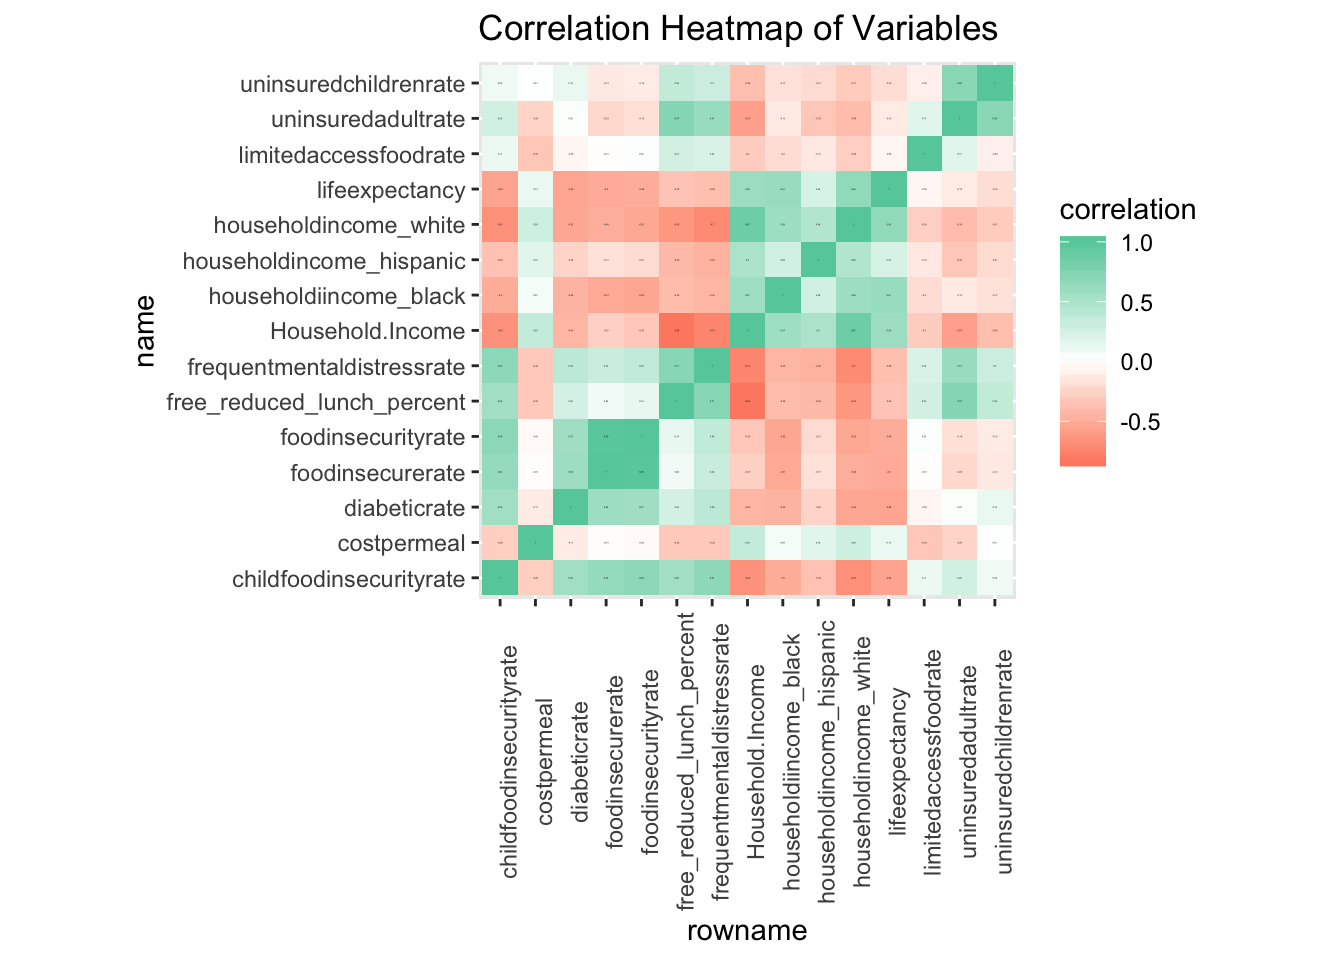
\includegraphics{project1_files/figure-latex/unnamed-chunk-5-1} \end{center}

\begin{Shaded}
\begin{Highlighting}[]
\CommentTok{#Dot Plot for Percentage of Children on Free/Reduced Lunch and Household Income#}
\KeywordTok{library}\NormalTok{(ggplot2)}
\KeywordTok{ggplot}\NormalTok{(joindata, }\KeywordTok{aes}\NormalTok{(}\DataTypeTok{x=}\NormalTok{Household.Income, }
\DataTypeTok{y=}\NormalTok{free_reduced_lunch_percent, }\DataTypeTok{color=}\NormalTok{urbanization)) }\OperatorTok{+}
\KeywordTok{ggtitle}\NormalTok{(}\StringTok{"Children on Free/Reduced Lunch vs. Household Income"}\NormalTok{) }\OperatorTok{+}
\KeywordTok{labs}\NormalTok{(}\DataTypeTok{y=} \StringTok{"Children on Free/Reduced Lunch (%)"}\NormalTok{, }
\DataTypeTok{x =} \StringTok{"Household Income ($)"}\NormalTok{) }\OperatorTok{+}\StringTok{ }
\KeywordTok{theme}\NormalTok{(}\DataTypeTok{legend.position =} \StringTok{"bottom"}\NormalTok{) }\OperatorTok{+}
\KeywordTok{geom_point}\NormalTok{(}\DataTypeTok{size=}\DecValTok{1}\NormalTok{, }\DataTypeTok{shape=} \DecValTok{5}\NormalTok{) }\OperatorTok{+}\StringTok{ }
\KeywordTok{geom_smooth}\NormalTok{(}\DataTypeTok{method=}\StringTok{'lm'}\NormalTok{, }\DataTypeTok{formula=}\NormalTok{y}\OperatorTok{~}\NormalTok{x) }\OperatorTok{+}\StringTok{ }
\KeywordTok{scale_y_continuous}\NormalTok{(}\DataTypeTok{lim=}\KeywordTok{c}\NormalTok{(}\DecValTok{0}\NormalTok{,}\DecValTok{100}\NormalTok{))}\OperatorTok{+}\StringTok{ }
\KeywordTok{scale_x_continuous}\NormalTok{(}\DataTypeTok{labels =} \ControlFlowTok{function}\NormalTok{(x) }\KeywordTok{format}\NormalTok{(x, }\DataTypeTok{scientific =} \OtherTok{FALSE}\NormalTok{))}\OperatorTok{+}
\KeywordTok{scale_color_brewer}\NormalTok{(}\DataTypeTok{palette =} \StringTok{"Set2"}\NormalTok{) }\OperatorTok{+}\StringTok{ }\KeywordTok{labs}\NormalTok{(}\DataTypeTok{color=} \StringTok{"Urbanization Status"}\NormalTok{)}
\end{Highlighting}
\end{Shaded}

\begin{center}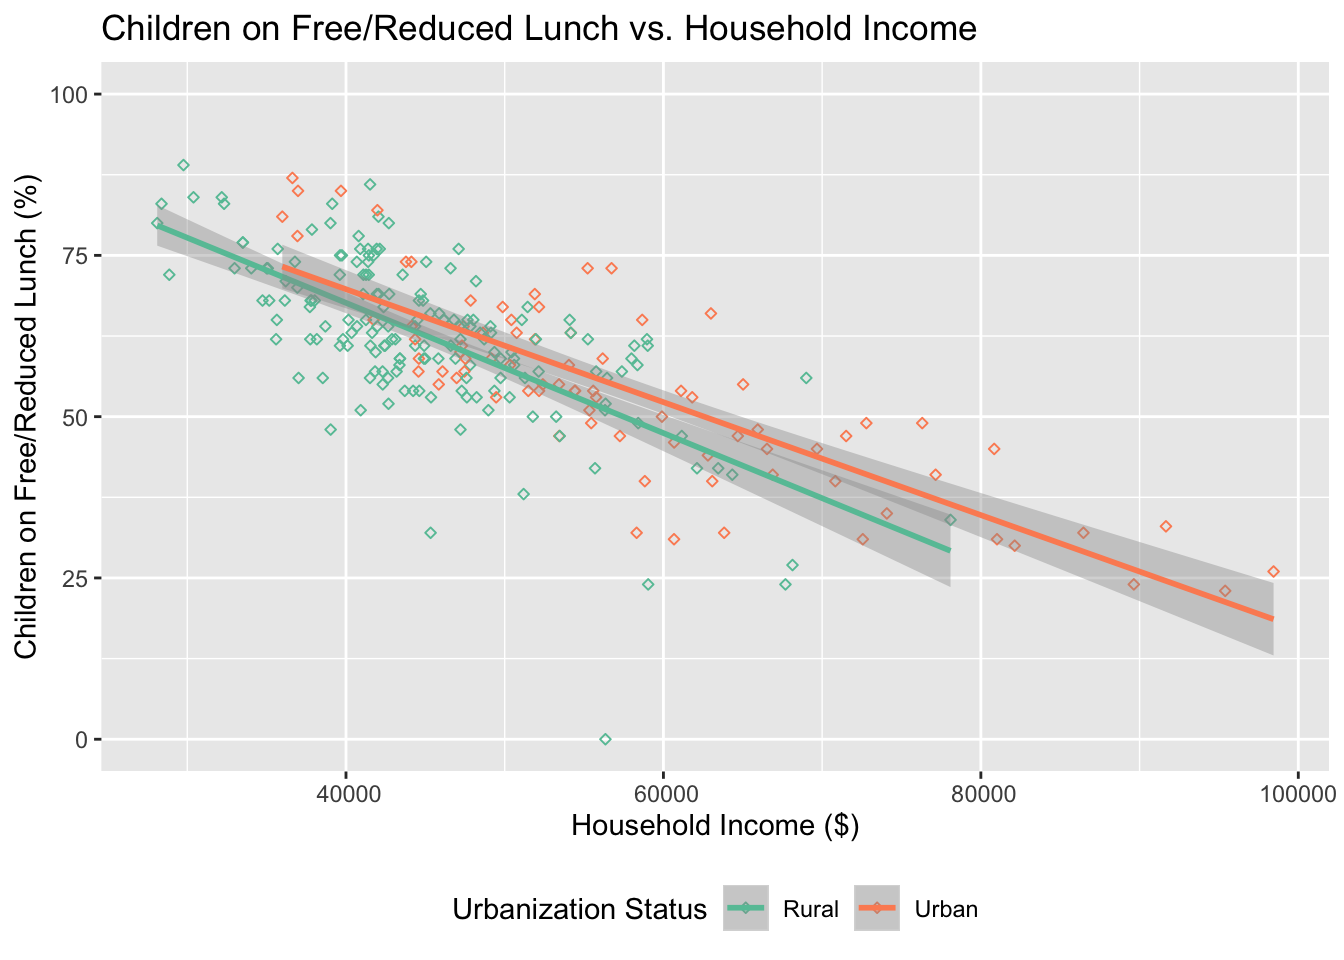
\includegraphics{project1_files/figure-latex/unnamed-chunk-5-2} \end{center}

\begin{Shaded}
\begin{Highlighting}[]
\CommentTok{#Bar Plot of Mean Life Expectancy By Border Status#}
\KeywordTok{library}\NormalTok{(ggplot2)}
\KeywordTok{ggplot}\NormalTok{(joindata, }\KeywordTok{aes}\NormalTok{(}\DataTypeTok{x=}\NormalTok{border_status, }\DataTypeTok{y=}\NormalTok{lifeexpectancy,}
\DataTypeTok{color=}\NormalTok{urbanization)) }\OperatorTok{+}\KeywordTok{scale_color_manual}\NormalTok{(}\DataTypeTok{values=}\KeywordTok{c}\NormalTok{(}\StringTok{"#CC66CC"}\NormalTok{, }\StringTok{"#6699FF"}\NormalTok{))}\OperatorTok{+}
\KeywordTok{scale_fill_manual}\NormalTok{(}\DataTypeTok{values=}\KeywordTok{c}\NormalTok{(}\StringTok{"#CC66CC"}\NormalTok{, }\StringTok{"#6699FF"}\NormalTok{))}\OperatorTok{+}
\KeywordTok{geom_bar}\NormalTok{(}\KeywordTok{aes}\NormalTok{(}\DataTypeTok{y=}\NormalTok{lifeexpectancy,}\DataTypeTok{fill=}\NormalTok{ urbanization), }
\DataTypeTok{stat=}\StringTok{"summary"}\NormalTok{, }\DataTypeTok{fun.y=}\StringTok{"mean"}\NormalTok{, }\DataTypeTok{position=} \StringTok{"dodge"}\NormalTok{) }\OperatorTok{+}\StringTok{ }
\KeywordTok{scale_y_continuous}\NormalTok{(}\DataTypeTok{name=} \StringTok{"Mean Life Expectancy (years)"}\NormalTok{, }
\NormalTok{(}\DataTypeTok{breaks=}\KeywordTok{seq}\NormalTok{(}\DecValTok{0}\NormalTok{,}\DecValTok{150}\NormalTok{, }\DecValTok{25}\NormalTok{)), }\DataTypeTok{lim=}\KeywordTok{c}\NormalTok{(}\DecValTok{0}\NormalTok{,}\DecValTok{100}\NormalTok{))}\OperatorTok{+}
\KeywordTok{ggtitle}\NormalTok{(}\StringTok{"Mean Life Expectancy By Border Status"}\NormalTok{) }\OperatorTok{+}
\KeywordTok{xlab}\NormalTok{(}\StringTok{"Border Status"}\NormalTok{)}\OperatorTok{+}
\KeywordTok{theme}\NormalTok{(}\DataTypeTok{legend.position =} \StringTok{"bottom"}\NormalTok{) }\OperatorTok{+}
\KeywordTok{labs}\NormalTok{(}\DataTypeTok{color=} \StringTok{"Urbanization Status"}\NormalTok{) }\OperatorTok{+}
\KeywordTok{labs}\NormalTok{(}\DataTypeTok{fill=} \StringTok{"Urbanization Status"}\NormalTok{)}
\end{Highlighting}
\end{Shaded}

\begin{center}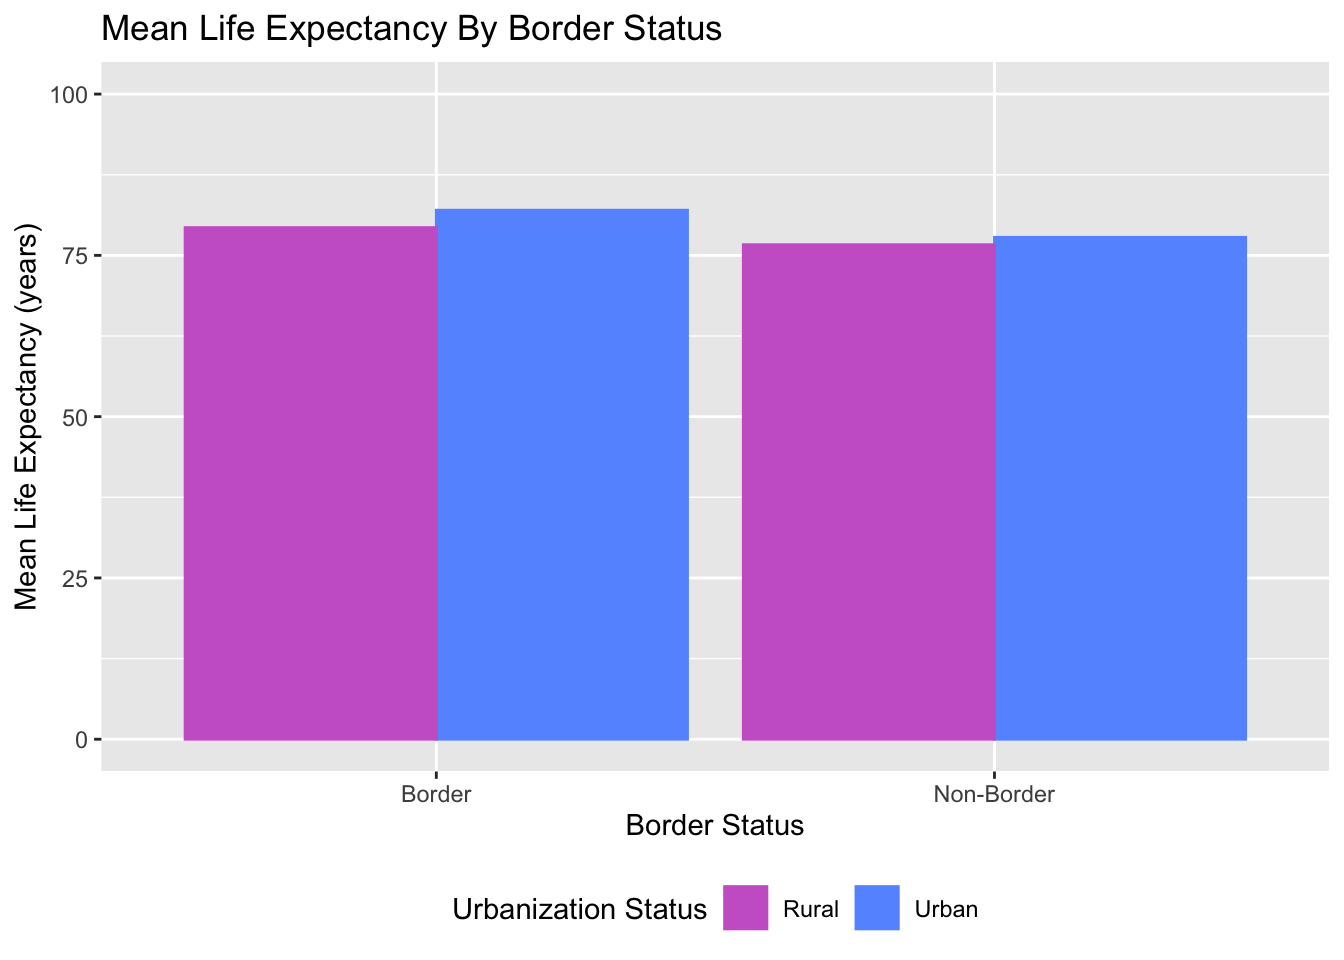
\includegraphics{project1_files/figure-latex/unnamed-chunk-5-3} \end{center}

\emph{The Correlation Heatmap shows that there is an obvious correlation
of 1 among each variable and itself. The rest of the table gives small
boxes with a value for the correlation between the two given numeric
variables at a given coordinate. I can see that there is a strong
negative correlation between household income and the percentage of
children in the county on free/reduced lunch. Moreover, there is also a
strong negative correlation between household income across all races
and child food insecurity rates. Looking at positive correlations, I can
see that there is a positive correlation between the rate of uninsured
adults and frequent mental distress. There is also a stronger
correlation between the rate of uninsured adults and the percentage of
children in the county on free/reduced lunch. I can also see, as
predicted in my Introduction, that there is a positive correlation
between child food insecurity rate and the percentage of children on
free/reduced lunches.}

\emph{The Dot Plot shows the relationship between household income and
the percentage of children on free/reduced lunch. As we can clearly see,
there is a negative linear relationship between the two variables, such
that as household income increases, the percentage of children on
free/reduced lunch decreases. Furthermore, we can see that the slope of
this relationship is even steeper for children in rural counties,
showing that the percentage of children on free/reduced lunch drops off
more steeply as household income increases, as compared to urban
counties.}

\emph{The Bar Plot shows how the mean life expectancy differs based on
border status and by urbanization status of counties. Interestingly
enough, the data show that the life expectancy is actually slightly
higher in counties that are classified as border communities and also
slightly higher in border regions classified as ``Urban''. This is the
opposite result as many would think, as accessibility to healthcare is
often harder to come by in border regions. Because there have not been
any tests for the statistical significance of these differences, I
cannot be sure that life expectancy among border and non-border counties
differs significantly.}

\#Dimensionality Reduction

\begin{Shaded}
\begin{Highlighting}[]
\KeywordTok{library}\NormalTok{(cluster)}
\NormalTok{pam_data <-joindata}\OperatorTok\StringTok{ }\KeywordTok{select}\NormalTok{(lifeexpectancy, foodinsecurerate, Household.Income)}
\NormalTok{sil_width <-}\KeywordTok{vector}\NormalTok{()}
\ControlFlowTok{for}\NormalTok{ (i }\ControlFlowTok{in} \DecValTok{2}\OperatorTok{:}\DecValTok{10}\NormalTok{) \{}
\NormalTok{  pam_fit <-}\StringTok{ }\KeywordTok{pam}\NormalTok{(pam_data, }\DataTypeTok{k=}\NormalTok{i)}
\NormalTok{  sil_width[i] <-pam_fit}\OperatorTok{$}\NormalTok{silinfo}\OperatorTok{$}\NormalTok{avg.width}
\NormalTok{\}}
\KeywordTok{ggplot}\NormalTok{()}\OperatorTok{+}\KeywordTok{geom_line}\NormalTok{(}\KeywordTok{aes}\NormalTok{(}\DataTypeTok{x=}\DecValTok{1}\OperatorTok{:}\DecValTok{10}\NormalTok{,}\DataTypeTok{y=}\NormalTok{sil_width))}\OperatorTok{+}
\KeywordTok{scale_x_continuous}\NormalTok{(}\DataTypeTok{name=}\StringTok{"k"}\NormalTok{,}\DataTypeTok{breaks=}\DecValTok{1}\OperatorTok{:}\DecValTok{10}\NormalTok{) }\OperatorTok{+}
\KeywordTok{ggtitle}\NormalTok{(}\StringTok{"Silhouette Width vs Number of Clusters in PAM"}\NormalTok{)}
\end{Highlighting}
\end{Shaded}

\begin{center}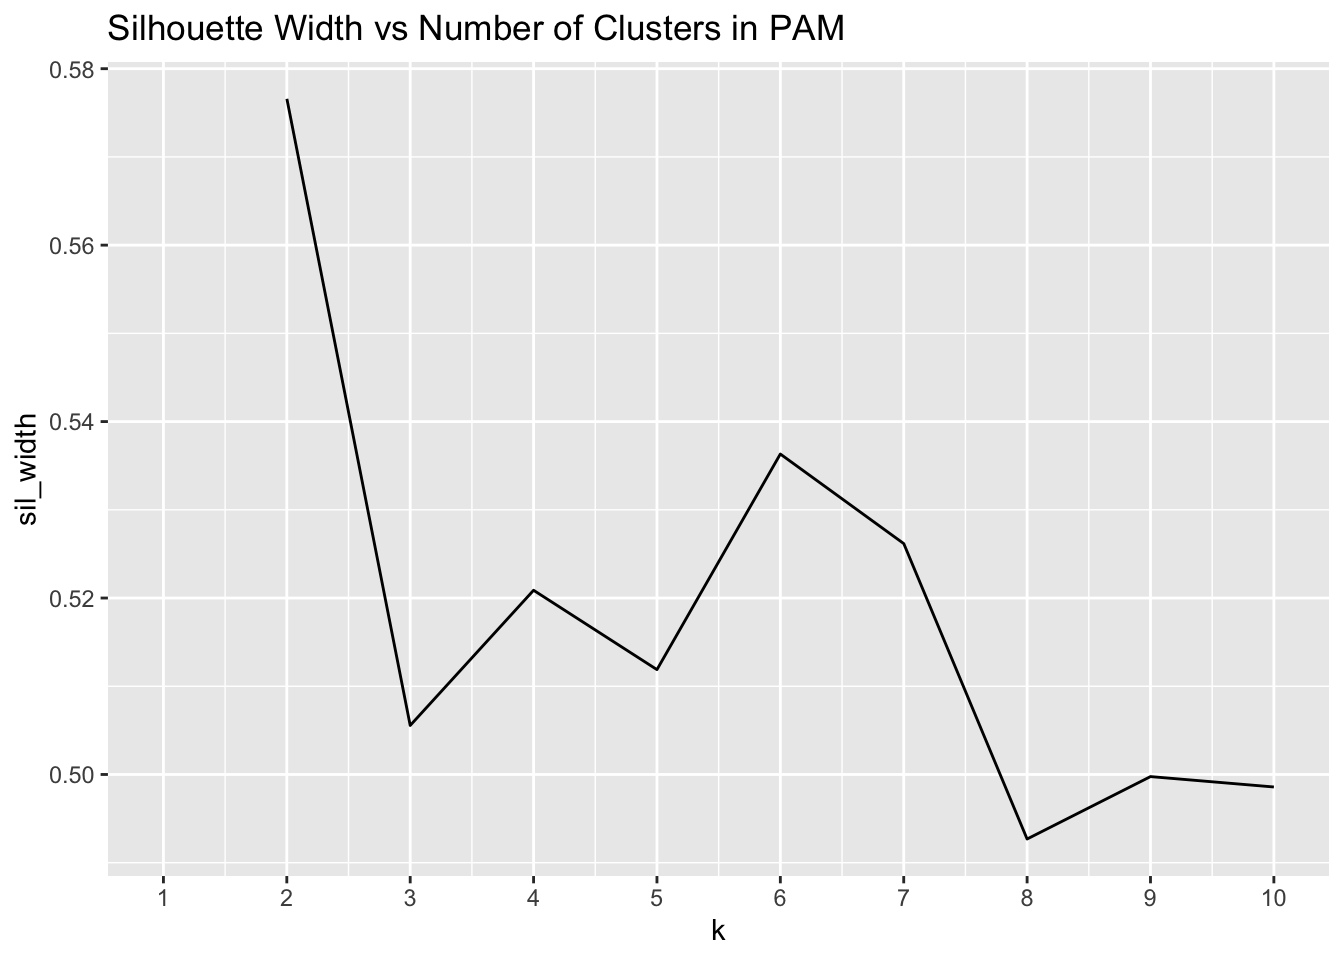
\includegraphics{project1_files/figure-latex/unnamed-chunk-6-1} \end{center}

\begin{Shaded}
\begin{Highlighting}[]
\NormalTok{pam2 <-}\StringTok{ }\NormalTok{joindata }\OperatorTok\StringTok{ }
\KeywordTok{select}\NormalTok{(lifeexpectancy, foodinsecurerate,}
\NormalTok{Household.Income)}\OperatorTok\StringTok{ }\KeywordTok{pam}\NormalTok{(}\DecValTok{2}\NormalTok{)}
\NormalTok{pam2}
\end{Highlighting}
\end{Shaded}

\begin{verbatim}
## Medoids:
##       ID lifeexpectancy foodinsecurerate Household.Income
## [1,] 136           81.4               10            42650
## [2,] 251           77.7                7            58363
## Clustering vector:
##   [1] 1 2 1 1 2 2 1 2 1 2 2 1 1 2 2 2 2 1 1 2 1 1 1 1 1 1 2 2 2 1 1 1 2 1 1 2 1
##  [38] 1 2 1 1 1 2 1 1 2 1 1 2 2 1 2 1 1 1 1 2 1 1 1 2 1 1 1 1 1 1 2 1 2 1 1 1 2
##  [75] 2 1 1 1 2 1 1 1 2 2 1 2 2 2 1 1 2 1 1 2 1 1 1 2 1 2
##  [ reached getOption("max.print") -- omitted 154 entries ]
## Objective function:
##    build     swap 
## 6019.958 5348.823 
## 
## Available components:
##  [1] "medoids"    "id.med"     "clustering" "objective"  "isolation" 
##  [6] "clusinfo"   "silinfo"    "diss"       "call"       "data"
\end{verbatim}

\begin{Shaded}
\begin{Highlighting}[]
\NormalTok{pam2}\OperatorTok{$}\NormalTok{silinfo}\OperatorTok{$}\NormalTok{avg.width}
\end{Highlighting}
\end{Shaded}

\begin{verbatim}
## [1] 0.5765833
\end{verbatim}

\begin{Shaded}
\begin{Highlighting}[]
\NormalTok{finalclust <-joindata }\OperatorTok\StringTok{ }
\KeywordTok{mutate}\NormalTok{(}\DataTypeTok{cluster=}\KeywordTok{as.factor}\NormalTok{(pam2}\OperatorTok{$}\NormalTok{clustering))}
\NormalTok{confmat3<-}\StringTok{ }\NormalTok{finalclust}\OperatorTok\StringTok{ }\KeywordTok{group_by}\NormalTok{(border_status)}\OperatorTok
\KeywordTok{count}\NormalTok{(cluster)}\OperatorTok\StringTok{ }\KeywordTok{arrange}\NormalTok{(}\KeywordTok{desc}\NormalTok{(n))}\OperatorTok
\KeywordTok{pivot_wider}\NormalTok{(}\DataTypeTok{names_from =} \StringTok{"cluster"}\NormalTok{, }
\DataTypeTok{values_from =} \StringTok{"n"}\NormalTok{, }\DataTypeTok{values_fill =} \KeywordTok{list}\NormalTok{(}\StringTok{'n'}\NormalTok{=}\DecValTok{0}\NormalTok{))}

\KeywordTok{ggplot}\NormalTok{(finalclust, }\KeywordTok{aes}\NormalTok{(}\DataTypeTok{x=}\NormalTok{lifeexpectancy,}
\DataTypeTok{y=}\NormalTok{foodinsecurerate, }\DataTypeTok{color=}\NormalTok{cluster))}\OperatorTok{+}\StringTok{ }\KeywordTok{geom_point}\NormalTok{()  }\OperatorTok{+}
\KeywordTok{ggtitle}\NormalTok{(}\StringTok{"Food Insecurity Rate vs Life Expectancy"}\NormalTok{) }\OperatorTok{+}
\KeywordTok{labs}\NormalTok{(}\DataTypeTok{y=} \StringTok{"Food Insecurity Rate (%)"}\NormalTok{, }
\DataTypeTok{x =} \StringTok{"Life Expectancy (years)"}\NormalTok{) }\OperatorTok{+}\StringTok{ }
\KeywordTok{theme}\NormalTok{(}\DataTypeTok{legend.position =} \StringTok{"bottom"}\NormalTok{)}
\end{Highlighting}
\end{Shaded}

\begin{center}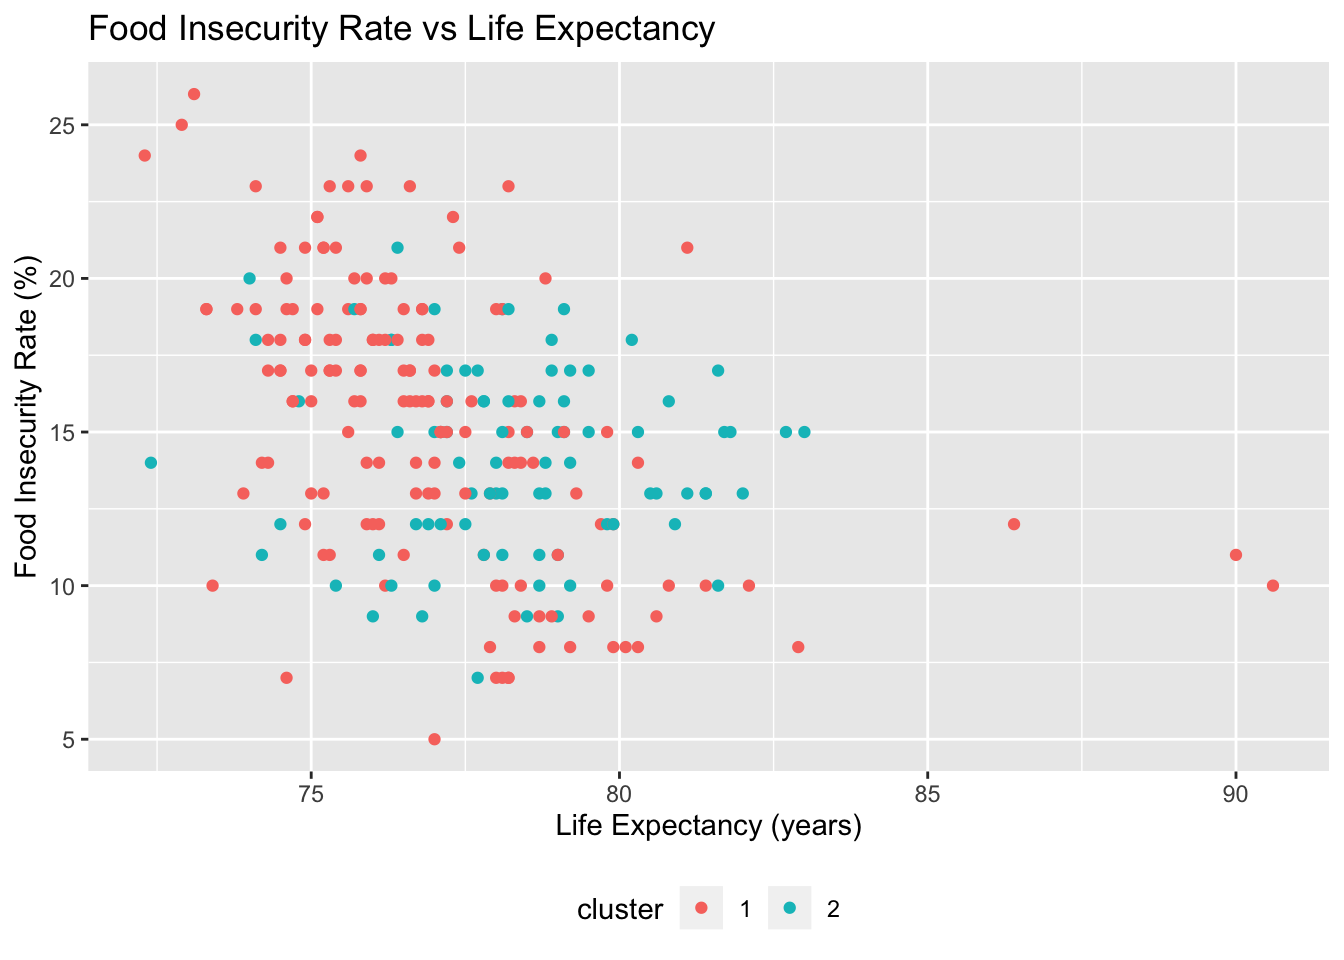
\includegraphics{project1_files/figure-latex/unnamed-chunk-6-2} \end{center}

\begin{Shaded}
\begin{Highlighting}[]
\KeywordTok{library}\NormalTok{(GGally)}
\KeywordTok{ggpairs}\NormalTok{(finalclust, }\DataTypeTok{columns =} \DecValTok{2}\OperatorTok{:}\DecValTok{5}\NormalTok{,}
\KeywordTok{aes}\NormalTok{(}\DataTypeTok{color=}\NormalTok{ cluster))}
\end{Highlighting}
\end{Shaded}

\begin{center}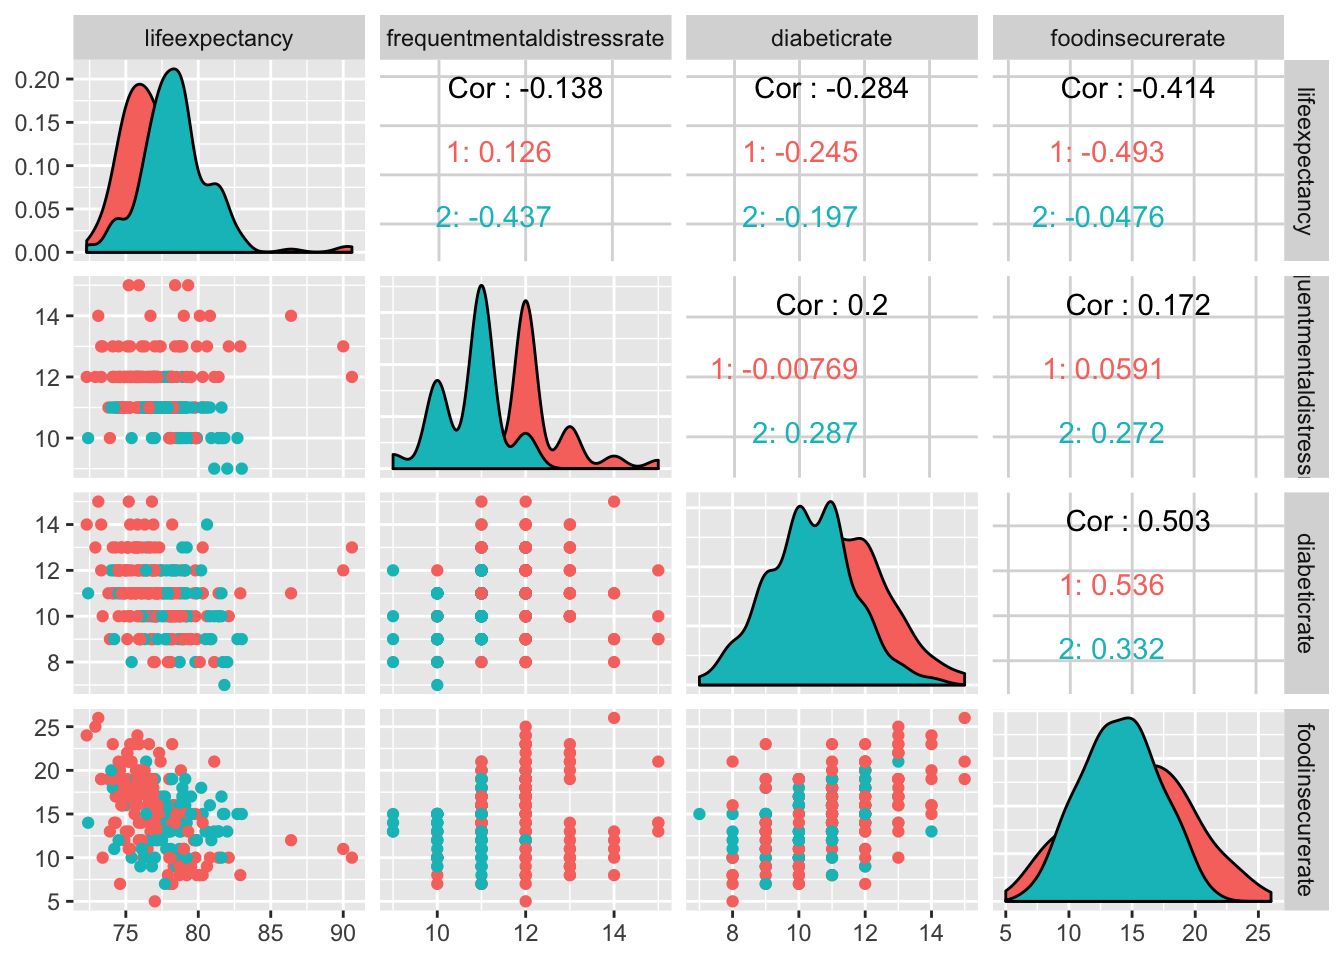
\includegraphics{project1_files/figure-latex/unnamed-chunk-6-3} \end{center}

\emph{By doing a Partitioning around Medoids, or PAM, method, I was able
to see how well the clusters that I made could partition my data. The
variables I wanted to visualize were Life Expectancy, Food Insecurity
Rate, and Household Income across the counties. I also used Border
Status to help visualize them through color. I chose the number of
clusters using a graph of average silhouette widths as a function of
cluster number. The graph indicated that the best number of clusters to
use is two because two clusters had the highest average silhouette width
at 0.5766 and is most parsimonious. This value indicates that I have
found a reasonable structure for partitioning my data, although it's not
necessarily classified as strong.}

\emph{It is rather apparent when looking at the visualization plot of
Food Insecurity Rate and Life Expectancy colored by cluster that the
data points are mixed together instead of occupying a visibly distinct
space for the given cluster. I then made a visualization of all the
pairwise combinations of four of my variables from my ``finalclust''
dataset, including Life Expectancy, Rate of Frequent Mental Distress,
Food Insecurity Rate, and Diabetic Rate, all colored by Border Status.
The variables that had the greatest correlation were Food Insecurity
Rate and Diabetic Rate at 0.503. This value is not a particularly strong
positive correlation. I could also see that there was a negative
correlation of -0.414 for Food Insecurity Rate and Life Expectancy. Many
of the other variables did not show particularly strong correlations
with one another, giving correlations of only +/- 0.1-0.2. It seems as
though the clusters that were made were not that effective, as many of
the data points remained mixed together. The Life Expectancy vs Food
Insecurity Rate plot showed the most effective clustering, although it
still didn't give distinct regions.}

\end{document}
